\author{\firstname{ }\lastname}

\begin{titlepage}
{\Large
\begin{center}
\vfill {RWTH AACHEN UNIVERSITY\\
        Chair of Information Systems\\
        Prof. Dr. Matthias Jarke}
% adapt kind of thesis
\vfill {\textbf{\ifdefined\BACHELOR Bachelor \else Master \fi Thesis \ifdefined\PROPOSAL
		\PROPOSAL
		\fi}}
% adapt title
\vfill {{\textbf{\thetitle}}}
% adapt personal information
\vfill {\theauthor\\
        Matr.-No. \matrNo\\
        Study-Program: Computer Science \ifdefined\BACHELOR B.Sc. \else M.Sc. \fi\\
        \thedate}
\vfill {
\begin{tabular}{ll}

% adapt supervisors
Supervisors:			&	\firstsupervisor\\
                        &	\firstsupervisorchair\\
                        &	\firstadvisoruniversity\\
                        &\\
                        &	\secondsupervisor\\
                        &	\secondsupervisorchair\\
                        &	\secondsupervisoruniversity\\
                        &\\                        &\\
Advisors:				&	\firstadvisor\\
                        &	\firstadvisorchair\\
                        &	\firstadvisoruniversity\\
                        \ifdefined\secondadvisor
                        &\\
                        &	\secondadvisor\\
                        &	\secondadvisorchair\\
                        &	RWTH Aachen University
                        \fi
\end{tabular}}
\end{center}
}
\end{titlepage}
\ifdefined\PROPOSAL
\else
% adapt title
\blankpage{}
\newpage{}
\thispagestyle{empty} %get rid of header/footer for toc page
\begin{tikzpicture}
\node[inner sep=0pt] at (0,0) {
	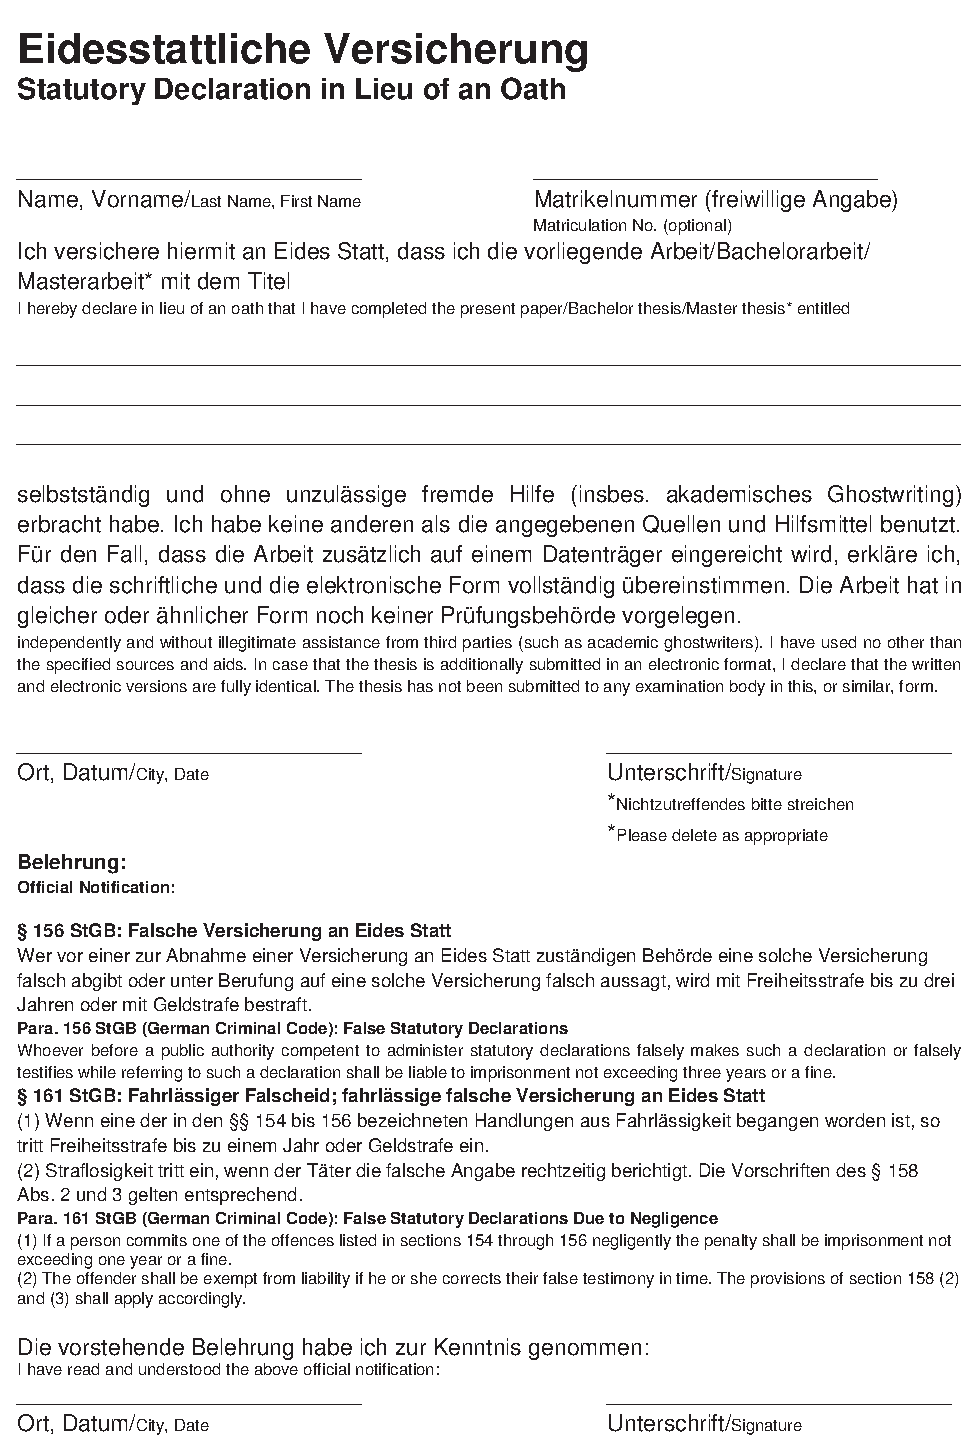
\includegraphics[width=\textwidth]{affidavit}
};
% name
\node[anchor=south west] at (-7.1,  8.2) {\lastname, \firstname};
% matr. no. OPTIONAL
\node[anchor=south west] at (0.6,  8.28) {\matrNo};
% title
\node[anchor=north west, align=left] at (-7.1,  6.0) {\thetitle};
% top date
\node[anchor=south west] at (-7.1,  -0.55) {Aachen, \thedate};
% bottom date
\node[anchor=south west] at (-7.1, -10.42) {Aachen, \thedate};
% program
\ifdefined\BACHELOR 
\draw ( 2.40, 7.2) -- ( 3.35, 7.2);
\draw ( -7.15, 6.76) -- ( -5.15, 6.76);
\else
\draw ( 2.40, 7.2) -- ( 5.70, 7.2);
\fi
\end{tikzpicture}

\fi